\section*{Instrucciones:}

La tarea se entrega y se resuelve en equipos de máximo 3 integrantes (1 a 3 personas). La tarea se entrega virtualmente en formato pdf tanto si son fotos de cuaderno, está realizada en word, en LATEX, etc.

No habrán reposiciones de tareas. Las tareas se pueden entregar con máximo 2 días de retraso para ser evaluadas sobre 8.

\textbf{Puntos Totales: 100}

\textbf{Tiempo estimado: $\approx$ 2hrs}

\section*{Ejercicios}

\begin{enumerate}
    \item Contesta de forma breve (máximo 3 líneas por pregunta) lo siguiente:

    \begin{enumerate}
        \item ¿Cuál es la diferencia entre una historia secuencial y una concurrente?

        Tomando como definición de historia como \textit{"una secuencia finita de eventos de invocación y de respuesta"}, lo que distancia a las historias secuenciales de las concurrentes es que las secuenciales forzosamente cada invocación se un método hace match enseguida con su respuesta, mientras que las concurrentes no cumplen en todos los casos esta regla. 
        
        \item Describe con tus propias palabras, ¿en qué consiste la linealizabilidad?

        La linealizabilidad es una propiedad dentro del mundo concurrente la cual nos permite asegurar que a pesar de que múltiples operaciones se puedan realizar de forma concurrente, el sistema se comportará como si estas operaciones se ejecutaran secuencialmente. 
        
        \item Describe con tus propias palabras, ¿cuál es la diferencia entre la consistencia secuencial y la linealizabilidad?

        La diferencia radica en que la consistencia secuencial requiere de mantener el orden de las operaciones (1 subhistoria por hilo) de cada hilo, mientras que para la linealizabilidad requiere mantener las precendencia de las operaciones a nivel global (historia completa).

        \hfill
    \end{enumerate}

    \item ¿La siguiente propiedad es equivalente a decir que un objeto x es wait-free?
    Argumenta por qué.

    \textbf{Propiedad:} Para toda historia infinita \texttt{H} de \texttt{x}, cada hilo que toma un número finito de pasos en \texttt{H} completa un número finito de llamadas a métodos.

    Esta definición es equivalente a \texttt{wait-free} ya que nos garantiza que cualquier elemento \texttt{x} en \texttt{H} con pasos finitos van a terminar los mismos, en esencia es la definición que tenemos de \texttt{wait-free} es el algoritmo que nos garantiza que cada llamada termina su ejecución en un número finito de pasos. Además de que cumple la definición de ser no bloqueante. Esto significa que los hilos o en este caso que cada elemento de \texttt{x} es no retrasara a los demás elementos de \texttt{H}. esto porque siempre realizara un numero finito de pasos para terminar de ejecutar un número finito de llamadas a métodos.

    Por lo que si esta propiedad nos dice que \texttt{x} terminara sus llamadas en un número finito de pasos es equivalente a la que \texttt{x} es \texttt{wait-free}.
    
    \hfill

    \item Considera la siguiente ejecución de una implementación de una pila para tres hilos p, q, r y sobre un solo objeto (de tipo pila).
    
    La especificación secuencial de una pila es que el método push(x) añade a x al inicio de la pila y el método pop() : x elimina el primer elemento x al inicio de la pila (mantiene \textit{LIFO}).

    \begin{center}
        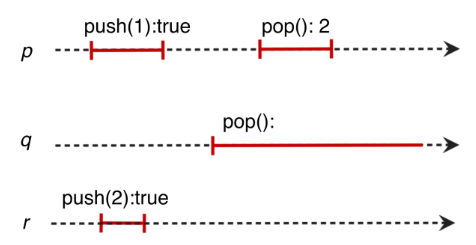
\includegraphics[width = 12 cm]{Images/Pregunta3_3.png}
    \end{center}

    \begin{enumerate}
        \item ¿Es linealizable con respecto a una pila? De ser así, incluye una 
        linearización y especifica la extensión de H y complete(H').

        \hfill

        \item ¿Es secuencialmente consistente? Incluye una historia que lo justifique.

        \hfill

        \item ¿Es consistente en la inactividad? Incluye una historia que lo justifique.

        \hfill
        
    \end{enumerate}

    \item Considera la siguiente ejecución de una implementación de una pila para dos hilos p, q y sobre dos objetos (de tipo pila) A, B. (Considera la especificación secuencial del ejercicio 2)

    \begin{center}
        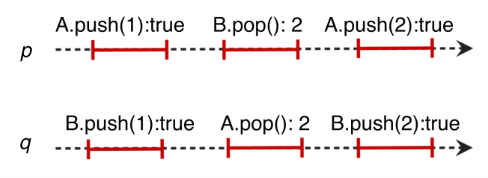
\includegraphics[width = 12 cm]{Images/Pregunta4_3.png}
    \end{center}

    \begin{enumerate}
        \item Considera que H es la historia de la ejecución, ¿H$\vert$A y H$\vert$B son secuencialmente consistentes?

        \hfill

        \item Considera que H es la historia de la ejecución, ¿H$\vert$A y H$\vert$B son linealizables?

        \hfill

        \item ¿La historia H es secuencialmente consistente y linealizable?

        \hfill
    \end{enumerate}

    \item Considera la siguiente clase \textit{Visibility}:

    \begin{center}
        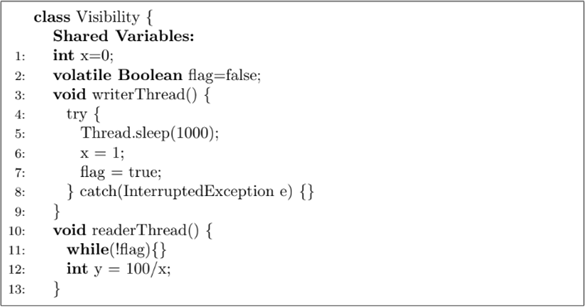
\includegraphics[width = 12 cm]{Images/Pregunta5_3.png}
    \end{center}

    \begin{enumerate}
        \item ¿Es posible que el método readerThread() divida entre cero? Argumenta porqué.

        Sí, es posible que el método \texttt{readerThread()} divida entre cero.\\

        \textbf{Explicación:}

        En el código solo la variable \texttt{flag} está declarada como \texttt{volatile}, mientras que \texttt{x} no lo está. Esto puede causar problemas de visibilidad debido al modelo de memoria de Java.
        
        \begin{itemize}
            \item Aunque el hilo escritor asigna \texttt{x = 1} antes de \texttt{flag = true}, el hilo lector puede ver el cambio en \texttt{flag} sin necesariamente ver el cambio en \texttt{x}. Esto se debe a que, sin la palabra clave \texttt{volatile} en \texttt{x}, no hay garantía de que el valor actualizado de \texttt{x} sea visible para otros hilos en el momento en que leen \texttt{flag}.
        
            \item El compilador y la CPU pueden reordenar las instrucciones para optimizar el rendimiento. Sin \texttt{volatile}, no hay garantías sobre el orden en que las escrituras a \texttt{x} y \texttt{flag} serán visibles para otros hilos.
        \end{itemize}
        
        El hilo lector puede salir del bucle \texttt{while(!flag){}} al ver \texttt{flag = true}, pero aún puede leer el valor antiguo de \texttt{x = 0}. Al ejecutar \texttt{int y = 100 / x;}, si \texttt{x} es \texttt{0}, se producirá una división por cero, lanzando una \texttt{ArithmeticException}.\\

        \item Si ambas variables son volatile, ¿es posible que el método readerThread() divida entre cero?
        
        Argumenta porqué.

        No, no es probable que el método \texttt{readerThread()} divida entre cero si ambas variables son \texttt{volatile}.\\

        \textbf{Explicación:}
        \begin{itemize}
            \item En Java, la palabra clave \texttt{volatile} asegura que las operaciones de lectura y escritura sean atómicas y proporciona garantías de visibilidad y ordenamiento de memoria.
        
            \item Cuando un hilo escribe en una variable \texttt{volatile} y otro hilo lee esa misma variable, se establece una relación de "sucede antes" \textit{(happens-before)}. Esto significa que todas las escrituras realizadas antes de escribir en la variable \texttt{volatile} son visibles para el hilo que lee después la misma variable \texttt{volatile}.
        \end{itemize}
        
        \textbf{Aplicación al código:}
        
        \begin{itemize}
        \item El hilo escritor asigna \texttt{x = 1;} seguido de \texttt{flag = true;}.
        \item Como ambas variables son \texttt{volatile}, cuando el hilo lector ve \texttt{flag = true}, también garantiza que verá \texttt{x = 1}.
        \end{itemize}
        
        El hilo lector no debería dividir entre cero porque \texttt{x} habrá sido actualizado a 1 antes de que \texttt{flag} sea visible como \texttt{true}. Por lo tanto, \texttt{int y = 100 / x;} se evaluará como \texttt{int y = 100 / 1;}, evitando la división por cero.\\

        \item Si ninguna de las dos variables es volatile, ¿es posible que el método readerThread() divida entre cero? Argumenta porqué.

        Sí, es posible y más probable que el método \texttt{readerThread()} divida entre cero si ninguna de las dos variables es \texttt{volatile}.\\

        \textbf{Explicación:}
        \begin{itemize}
            \item Sin \texttt{volatile} no hay garantías sobre cuándo (o si) las actualizaciones a \texttt{x} y \texttt{flag} serán visibles para otros hilos. El hilo lector puede no ver nunca las actualizaciones realizadas por el hilo escritor, o verlas en un orden diferente.
        
            \item El compilador o el procesador pueden reordenar las instrucciones, lo que significa que el hilo escritor podría, desde la perspectiva del hilo lector, asignar primero \texttt{flag = true} antes de \texttt{x = 1}.
        \end{itemize}
        
        \textbf{Consecuencia:}
        
        \begin{itemize}
            \item El hilo lector puede salir del bucle \texttt{while(!flag){}} al ver un valor desactualizado de \texttt{flag} o nunca salir del bucle si no ve el cambio.
            \item Si sale del bucle y \texttt{x} aún es \texttt{0} (porque no ha visto la actualización), al ejecutar \texttt{int y = 100 / x;}, se producirá una división por cero.
        \end{itemize}
         Se podría dar el caso que el hilo lector entre en un bucle infinito si nunca ve el cambio en \texttt{flag}, ya que no es \texttt{volatile}.
            \end{enumerate}
    
\end{enumerate}
